%% ICRA submission draft -- IEEE conference template (ieeeconf.cls from ras.papercept.net)
%% Compile on Overleaf with pdfLaTeX + BibTeX.  Status: FIRST DRAFT, simulation results only.
\documentclass[letterpaper, 10 pt, conference]{ieeeconf}

\IEEEoverridecommandlockouts
\overrideIEEEmargins

\usepackage{graphicx}
\usepackage{amsmath,amssymb}
\usepackage{booktabs}
\usepackage{cite}
\usepackage{url}
\usepackage{xcolor}
\usepackage[caption=false,font=footnotesize]{subfig}

\newcommand{\todo}[1]{\textcolor{red}{[TODO: #1]}}
\newcommand{\unit}[1]{\,\mathrm{#1}}

\title{\LARGE \bf
Grasp, Lift and Turn: Contact-Rich Leaf Presentation for Illumination-Robust Colour Inspection with a Mobile Manipulator}

\author{Yogesh Chawla$^{1}$% <-this % stops a space
\thanks{$^{1}$Y. Chawla is with \todo{affiliation}. {\tt\small yogeshchawla2850@gmail.com}}%
\thanks{\todo{Add co-authors, affiliations and funding.}}%
}

\begin{document}
\maketitle
\thispagestyle{empty}
\pagestyle{empty}

%% ---------------------------------------------------------------------------
\begin{abstract}
Leaf colour is an inexpensive proxy for crop nutrient status, but field measurements from
cameras are confounded by illumination, viewing angle and occlusion. We present a mobile
manipulation pipeline that makes the measurement physical: the robot drives to a plant,
pinches a leaf blade under force regulation with a two-finger gripper, lifts and rolls it in
front of a wrist camera that does not move with the gripper, and compares the presented
blade against a colour-reference board mounted on the platform and observed under the same
illuminant. Navigation and leaf targeting use only an RGB-D camera on the platform: the
nearest plant in the row is located by back-projected leaf-coloured points, and pinch
patches are found by plane fits on the leaf point cloud with reachability and clearance
scoring. A rotary tool joint between the flange bracket, which carries the camera, and the
gripper realises the turn while the camera stays still. We evaluate the pipeline in a
physics simulation of a finite-element maize plant in a planted field. Over the reported
runs the platform parks within 1.5\,cm of its goal, all selected leaves are pinched and held
for the required time at a regulated 3--4\,N with no force-safety trips, and the
chromaticity verdict matches the true leaf class for every green/dark-green leaf; adjacent
shades remain ambiguous. We also report a negative result: a two-finger pinch cannot twist a
stiff blade unless pad width, pinch force, leaf stiffness and pinch location along the
blade satisfy a torque budget, which we quantify.
\end{abstract}

%% ---------------------------------------------------------------------------
\section{Introduction}

Chlorophyll content, and with it nitrogen status, changes leaf colour long before yield is
affected, and hand-held meters such as the SPAD-502 exploit this~\cite{markwell1995}.
Cameras could make the measurement continuous and cheap, but a leaf imaged in the field is
lit by a mixture of direct sun and sky, seen at an uncontrolled angle, partly shadowed and
often occluded by its neighbours. Image-based chlorophyll estimation therefore relies on
careful radiometric calibration~\cite{wang2014} and still degrades away from the
conditions it was fitted for.

Ground robots that touch the plant can remove these confounds instead of modelling
them. Sensorised leaf grippers have been used to clamp a blade for contact
measurements~\cite{atefi2019}, and manipulators have picked leaves under visual
servoing~\cite{ahlin2016}. What has not been shown, to our knowledge, is the loop in which
the robot \emph{presents} a leaf to its own camera under regulated contact while the same
camera, or a co-located one, sees a colour reference under the same illuminant, so that the
colour verdict is a relative measurement rather than an absolute one.

This paper describes such a system and the design decisions that made it work in a
contact-rich simulation (Fig.~\ref{fig:overview}):
\begin{itemize}
\item a mobile platform with a single 7-DoF arm and a two-finger gripper on a rotary tool
joint, a colour board fixed to the platform, and three RGB-D cameras (navigation, scene,
wrist);
\item navigation and leaf targeting from the RGB-D data alone, with simulator ground truth
used only to grade results;
\item a pinch controller that closes on force, re-centres the gripper on the blade, then
lifts and rolls it through $\pm35^\circ$ under a force limit while colour is sampled and
validated by depth; and
\item an analysis of when a pinched blade actually follows the gripper, which turned out to
be the hardest part of the problem.
\end{itemize}

All results are in simulation. We state this plainly because it shapes what can be
claimed: the contribution is the closed loop and its failure analysis, not field
performance.

\begin{figure}[t]
\centering
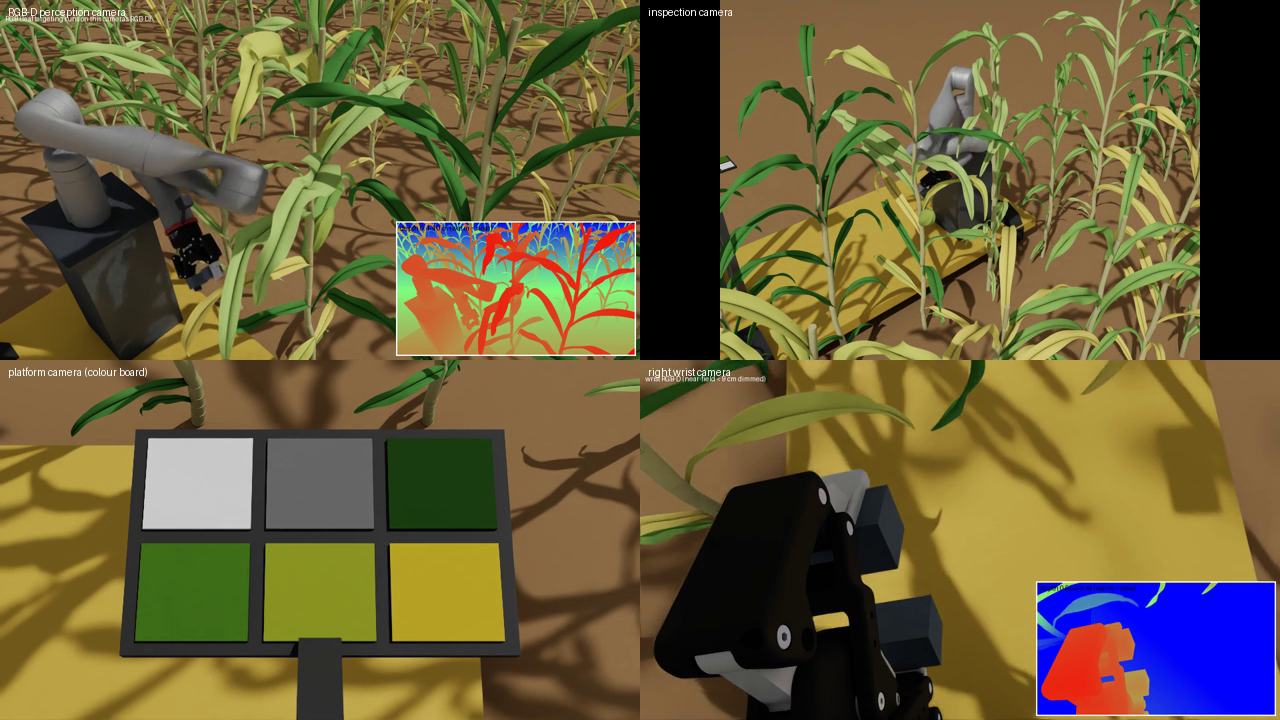
\includegraphics[width=\columnwidth]{figs/overview_crop.png}
\caption{The system in the simulated field. Top left: platform RGB-D perception camera
(depth inset) after the drive-in; top right: canopy camera showing the arm reaching into
the first row; bottom left: the fixed colour board seen by its own camera; bottom right:
the wrist RGB-D camera on the flange bracket, looking at the pads.}
\label{fig:overview}
\end{figure}

%% ---------------------------------------------------------------------------
\section{Related Work}

\textbf{Plant phenotyping robots.} The Robotanist~\cite{muellersim2017} established the
pattern of a row-following ground platform with a manipulator for contact measurements in
sorghum. Atefi et al.~\cite{atefi2019} clamp maize and sorghum leaves with a sensorised
gripper to read chlorophyll and temperature in vivo. Ahlin et al.~\cite{ahlin2016} pick
leaves with a manipulator using learned detection and visual servoing. These systems either
measure at the point of contact or remove the leaf; none use the contact to control what
a camera sees.

\textbf{Colour references.} Reference charts~\cite{mccamy1976} are standard in imaging
phenotyping, but they are usually placed in the scene by hand and imaged separately from
the plant. Mounting the board on the platform and observing it continuously with its own
camera turns it into a live illuminant estimate.

\textbf{Deformable manipulation.} Leaves are thin, anisotropic shells attached to a
compliant stalk; grasping them is a deformable-object problem~\cite{sanchez2018} for
which simulation with finite-element bodies is now practical in GPU physics
engines~\cite{physx}. We build on Isaac Lab~\cite{mittal2023} and a maize plant cooked as a
volumetric FEM~\cite{plantrepo}.

\textbf{Row navigation.} Camera-based row following is well studied~\cite{bakker2011}; our
navigation is deliberately simple (nearest leaf cluster in the lane) because the
contribution lies elsewhere.

%% ---------------------------------------------------------------------------
\section{System}

\subsection{Platform and arm}
A wheeled platform (kinematic in simulation, holonomic) carries a pedestal with a Kinova
Gen3 7-DoF arm and, on the opposite side, a colour board on a post with a 26\,mm camera on a
mast 26\,cm above it. The board leans $35^\circ$ so that its face normal points straight
up when parked; its six patches are white, grey and four leaf shades from dark green to
yellow.

\subsection{Rotary tool joint and cameras}
The Robotiq 2F-85 gripper hangs from a bracket on the flange through an additional revolute
joint about the approach axis (Fig.~\ref{fig:overview}, bottom right). The 7-DoF inverse
kinematics positions the \emph{bracket}; the extra joint turns only the gripper. The wrist
RGB-D camera (14\,mm, $960{\times}540$) is mounted on the bracket 13\,cm above the pads and
8\,cm to the side, so the blade beside the pads fills the frame and the view does not move
when the gripper rolls. Two earlier designs failed: using the arm's seventh joint as the
roll with the camera on the preceding link stalled the IK against joint limits, and a
null-space bias could carry only a third of the roll because the arm's natural wrist angle
differs by $105^\circ$ between leaves at different heights. A forward-looking navigation
camera (10.5\,mm, pitched $30^\circ$ down) and a scene camera (16\,mm) sit on the mast.

\subsection{Fingertips}
Each inner finger carries a 2\,g load-cell pad ($40{\times}3{\times}26$\,mm) on a fixed joint
whose incoming joint force is the contact load, faced with a rubber physics material
($\mu_s=1.6$) and a 20\,mm visual rubber block. The blocks matter for interpretation: the
plant's collision envelope is about 4\,cm thick around a blade rendered a few millimetres
thick (Sec.~\ref{sec:plant}), so the load-cell faces stop 50\,mm apart while the rendered
blade sits in the middle.

\subsection{Plant and field}\label{sec:plant}
The target is a half-scale maize plant (stalk, 14 leaves, ear) cooked as hexahedral FEM
bodies at resolution 30, 128 solver iterations, 60\,Hz, following~\cite{plantrepo}; the
recipe only stands with a 3\,kg stalk mass override and runtime damping, which we keep
unchanged. Leaves carry five nominal sRGB shades as ground truth. The field has 314
visual-only copies in agronomic rows (0.75\,m between rows, 0.35\,m within a row); the target
is the first-row plant and the robot approaches across the open headland.

%% ---------------------------------------------------------------------------
\section{Method}

\subsection{Navigation}
While driving, the navigation camera is read at 3\,Hz. Leaf-coloured pixels
(hue $38$--$135^\circ$, saturation $>0.28$, value $>0.12$) are back-projected through the
depth image with the camera pose that follows from the platform's odometry and the fixed
mount, expressed in the platform frame, and restricted to the lane ahead ($|y|\le0.35$\,m,
$0.1$--$4.5$\,m out, $0.3$--$1.5$\,m up). The nearest 70\,cm-deep cluster along the row is the
plant and its median $xy$ the goal. Two rules were needed: once the plant is within 1\,m the
target is locked and estimates jumping more than 0.4\,m are rejected (otherwise, when the
plant leaves the near-range window, the ``nearest cluster'' becomes the next plant and the
platform drives through the target), and under 0.5\,m the estimate is frozen and odometry
finishes the approach (leaf tips reaching toward the camera bias the median by 20\,cm at
close range). The platform follows a decelerating profile in $x$ and a proportional lateral
correction until the plant sits at the origin of its frame within 3\,cm.

\subsection{Leaf targeting}
After arrival the scene camera provides one RGB-D frame. Rather than segmenting the image
(overlapping leaves merge into a single blob), the leaf point cloud is scanned directly:
every occupied 3\,cm voxel seeds a 4\,cm plane fit giving a patch centre (top surface) and
normal; the near-plane points within 12\,cm give the local blade axis, extent and droop
toward the stalk; clearance is counted in 1\,cm voxels against all other leaf points inside
the descent corridor, the sweep slab and the column above the patch. A patch is usable if
its normal is within $57^\circ$ of vertical, the blade extends away from the arm's side, the
patch and the pre-pinch point are within reach, droop is under 6\,cm, and fewer than 60
voxels obstruct. Blades must root within 18\,cm of the plant position found by navigation,
which excludes the in-row neighbours. Candidates are ranked by a score that rewards blade
length, distance out toward the tip and proximity, and up to $N$ targets are picked with
hues at least $10^\circ$ apart. At the pre-pinch point the wrist camera re-fits the patch
from close up (typical shift 8\,mm). Simulator nodes are used afterwards only to identify
the nearest true leaf and grade colour and deflection.

\subsection{Pinch, centring and presentation}
The gripper transits above the pre-pinch point (10\,cm from the patch on the approach side,
12\,cm up), descends, and slides across the blade with the pads open until they straddle
the patch. Closure is commanded as a normalised finger-joint target: it snaps to the gap
known from earlier holds, then creeps at $0.2\,\mathrm{s^{-1}}$ until the filtered pad load
reaches 0.15\,N, dwells 0.35\,s, and regulates the summed load to the target
(3--4\,N in the reported runs; 2--6\,N or 2.5--7\,N hold window; 7--8\,N trip). Because
closure is symmetric about the gripper axis but the blade surface estimate is coarse, one
pad always touches first; a centring admittance moves the whole gripper along the blade
normal toward the loaded pad at up to 1\,cm/s until both pads share the load. The hold then
lifts the blade up to 30\,mm and sweeps the roll $+35^\circ\to-35^\circ\to0$ at $8^\circ$/s,
both force-limited with hysteresis so a transient does not end the motion. A leaf is
complete after six seconds of continuous valid hold with at least three valid colour frames
and the finished sweep.

\subsection{Colour}
At 1\,Hz the wrist camera samples the blade 4--8\,cm from the pads (following the lifted
blade) and the board camera samples the six patches; samples are validated by projected
depth and, for the leaf, by the hue gate. A two-point white/grey calibration is chosen by
the residual on the colour patches, and the verdict is the swatch nearest in chromaticity,
reported with a separation margin; margins below 0.15 are flagged ambiguous. Only frames
from the current uninterrupted hold count.

%% ---------------------------------------------------------------------------
\section{Experiments}

All runs use Isaac Sim 6.0 / Isaac Lab~3 on one RTX~5090, 60\,Hz physics, 30\,Hz control,
headless with all cameras rendering; a two-leaf run takes 6--8\,min of wall time.

\subsection{Navigation}
From a start 2.5\,m behind and 0.25\,m beside the goal, the plant estimate in the odometry
frame stayed within 17\,mm of the true stalk from the first frame at 2.5\,m range, locked at
0.96\,m, and the platform parked at $(-1.1, +1.5)$\,cm from nominal in 6.1\,s (14 camera
updates). The same numbers reproduced across all later runs
($\le1.3$\,cm, $\le1.5$\,cm).

\subsection{Leaf targeting}
On the scene frame after arrival the scan produced 12 patch candidates of which 4 were
usable; the two chosen landed 3\,mm from the FEM leaves that the ground-truth targeting had
picked in earlier runs (Fig.~\ref{fig:detect}). With in-row neighbours 0.35\,m away and the
root-at-plant filter, all selected patches belonged to the target plant in every run.

\begin{figure}[t]
\centering
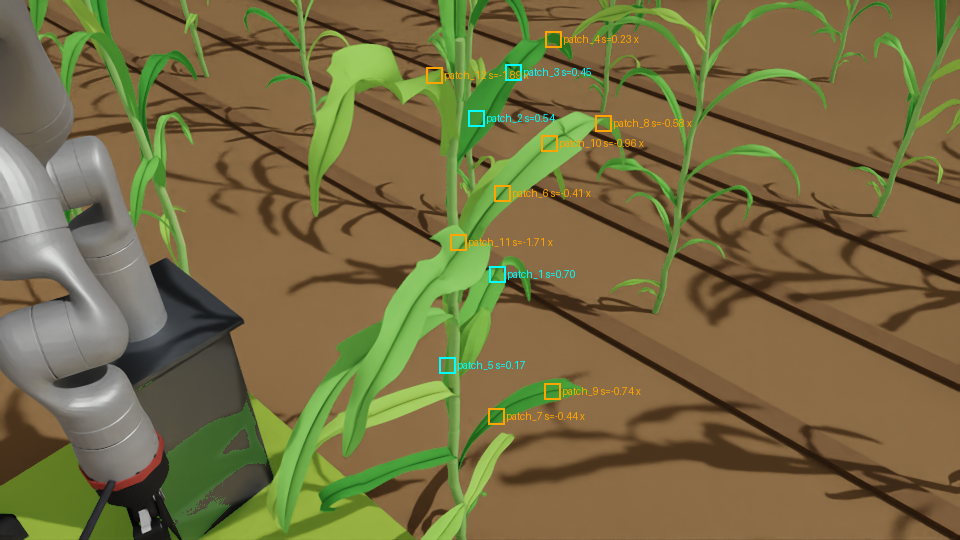
\includegraphics[width=\columnwidth]{figs/detections_rq17.png}
\caption{Scene-camera frame after arrival with the patch candidates (cyan usable, orange
rejected) found by the voxel-seeded plane-fit scan. Overlapping leaves defeat image-blob
segmentation; the scan works in the point cloud instead.}
\label{fig:detect}
\end{figure}

\subsection{Pinch, hold and colour}
Table~\ref{tab:runs} summarises representative runs. Every selected leaf was pinched,
centred and held for the required time; no force-safety trip occurred in these runs, and the
regulated load tracked its target within 0.1\,N. The chromaticity verdict matched the true
class for every green and dark-green leaf. Two failure modes are visible: the
\emph{yellow} leaf ties with \emph{yellow-green} (margin 0.03), and \emph{light green},
which lies between two swatches, lands on either neighbour. Sampling near the tip of a blade
also lowered the margin on one green leaf (0.09--0.13) compared with mid-blade sampling
(0.9). With the pads the rendered blade is visibly held (Fig.~\ref{fig:pads}).

\begin{table}[t]
\caption{Representative runs (simulation, camera-based targeting, autonomous drive). Pinch
is the mean summed pad load over the hold; ``turn'' is the rotation of the true blade normal
at the pinch during the $\pm35^\circ$ sweep.}
\label{tab:runs}
\centering
\footnotesize
\begin{tabular}{@{}lllcccl@{}}
\toprule
run & leaf (true class) & verdict & pinch & margin & turn & note \\
\midrule
rq22 & leaf\_2\_3 (green) & green & 3.0\,N & 0.11 & $21^\circ$ & 1e7\,Pa leaves \\
     & leaf\_4\_9 (dark green) & dark green & 3.1\,N & 0.98 & $0^\circ$ & \\
rq30 & leaf\_2\_3 (green) & green & 3.0\,N & 0.13 & $2^\circ$ & \\
     & leaf\_4\_9 (dark green) & dark green & 3.0\,N & 1.00 & $0^\circ$ & \\
     & leaf\_3\_9 (yellow) & yellow-green & 3.0\,N & 0.03 & $0^\circ$ & tie \\
rq33 & leaf\_2\_3 (green) & green & 4.1\,N & 0.11 & $7^\circ$ & 3e4\,Pa leaves, \\
     & leaf\_4\_3 (light green) & yellow-green & 4.0\,N & 0.41 & $43^\circ$ & 40\,mm pads \\
     & leaf\_4\_9 (dark green) & dark green & 4.3\,N & 0.99 & $0^\circ$ & \\
rq35 & leaf\_4\_3 (light green) & green & 4.0\,N & 0.09 & $3^\circ$ & field, canopy cam \\
     & leaf\_1\_3 (dark green) & dark green & 4.0\,N & 1.00 & $15^\circ$ & \\
     & leaf\_2\_3 (green) & green & 4.0\,N & 0.13 & $3^\circ$ & \\
\bottomrule
\end{tabular}
\end{table}

\begin{figure}[t]
\centering
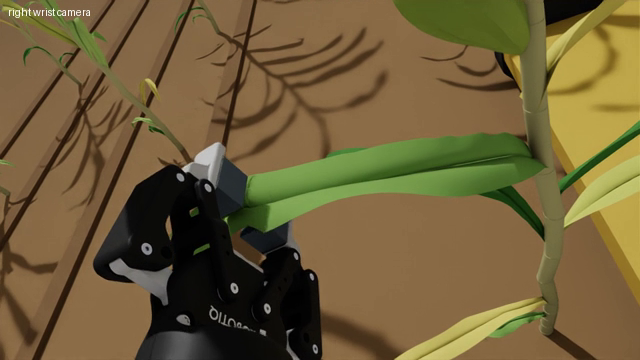
\includegraphics[width=\columnwidth]{figs/pads_crop.png}
\caption{Wrist camera during a hold at 3\,N: the rubber pad faces on the rendered blade
while the gripper rolls. The load-cell faces stop on the plant's 4\,cm collision envelope.}
\label{fig:pads}
\end{figure}

\subsection{When does the blade follow the gripper?}\label{sec:turn}
The roll is meant to show the camera both faces of the blade, and the ``turn'' column of
Table~\ref{tab:runs} is the honest measure of whether it does. With the original leaf
material (Young's modulus $10^7$\,Pa) the blade rotated $0$--$3^\circ$ regardless of pinch
force (0.7--3\,N), pad friction, pinch location (mid-blade or at 70--80\,\% toward the tip)
and roll axis (across the blade, or along it by approaching from the tip with the platform
driven in from the far end of the row). The reason is a torque budget. The pads transmit at
most $F\mu w/2\approx 3\times1.6\times0.011\approx0.05$\,N\,m with 22\,mm pads, whereas
twisting a $40{\times}14$\,mm section by $35^\circ$ over the 26\,mm pad length at
$10^7$\,Pa needs of order 2\,N\,m; torsional stiffness scales with the fourth power of the
section, so even 100$\times$ softer leaves ($10^5$\,Pa, stable in the plant-only settling
check, Table~\ref{tab:soft}) were still short by about $6\times$. Softening the leaves to
$3\times10^4$\,Pa (330$\times$), widening the pads to 40\,mm and raising the pinch to 4\,N
brought the budget to a margin of about 1.5 and produced the first visible turn: $42.8^\circ$
with 21\,mm of deflection on a light-green leaf pinched at 53\,\% of its length
(Fig.~\ref{fig:sweep}). Leaves pinched close to the sheath, where the section is thick,
still do not follow ($0$--$7^\circ$), which makes pinch location along the blade the
dominant variable.

\begin{table}[t]
\caption{Plant-only settling check with softened leaves (stalk unchanged): all nodes finite,
stalk top within 0.3\,mm of its cooked height, p95 node speed $<1.3$\,mm/s after 10\,s.}
\label{tab:soft}
\centering
\footnotesize
\begin{tabular}{@{}lccc@{}}
\toprule
leaf $E$ (Pa) & passed & stalk sag & leaf sag mean / max \\
\midrule
$2\times10^6$ & yes & 5\,mm & 19 / 66\,mm \\
$1\times10^6$ & yes & 5\,mm & 13 / 49\,mm \\
$1\times10^5$ & yes & 5\,mm & 13 / 33\,mm \\
$3\times10^4$ & yes & 5\,mm & 14 / 33\,mm \\
\bottomrule
\end{tabular}
\end{table}

\begin{figure}[t]
\centering
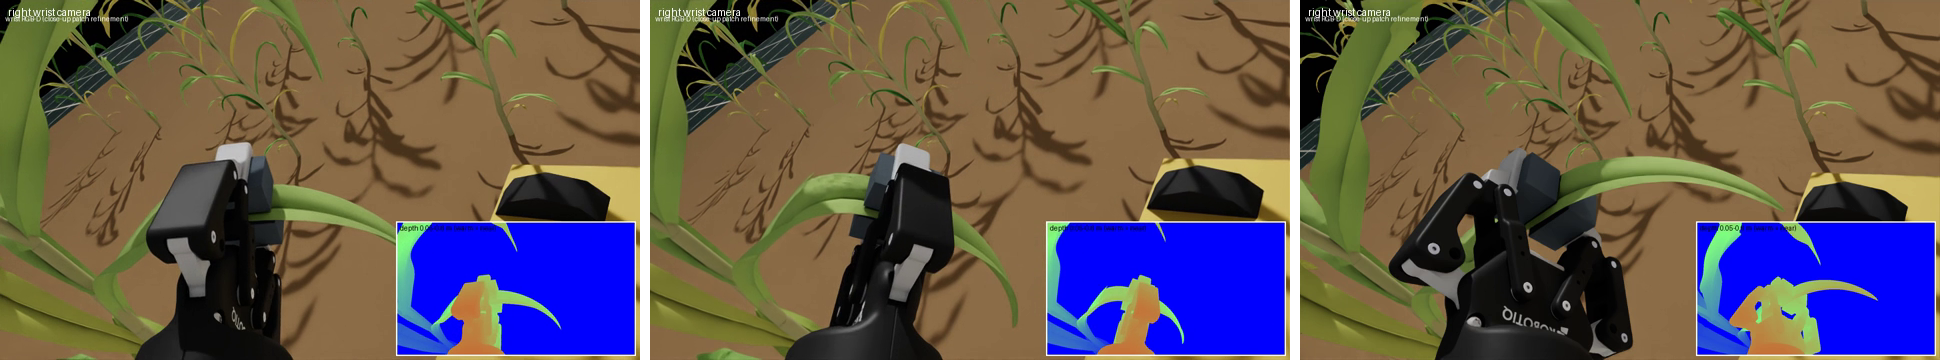
\includegraphics[width=\columnwidth]{figs/sweep_strip.png}
\caption{Wrist camera at roll $0^\circ$, $+35^\circ$ and $-35^\circ$ on the light-green leaf
of run rq33 (leaves at $3\times10^4$\,Pa, 40\,mm pads, 4\,N): the blade follows the pads
and its far end swings across the view.}
\label{fig:sweep}
\end{figure}

%% ---------------------------------------------------------------------------
\section{Discussion and Limitations}

\textbf{Simulation only.} Every number above comes from one plant model in one simulator.
The FEM plant's collision envelope is far thicker than a real blade, which both hides the
pads' true closure and exaggerates torsional stiffness; real maize blades twist easily near
the tip. The leaf segmentation is a hue gate that a real camera would not enjoy. The
colour ground truth is five painted shades, not chlorophyll or SPAD readings.

\textbf{What we believe transfers.} The force-then-centre pinch, the force-limited
presentation with the camera decoupled from the roll, the co-observed reference board and
the depth-validated sampling are hardware-agnostic and cheap; the torque budget of
Sec.~\ref{sec:turn} is a design rule for any leaf-handling end effector.

\textbf{Next.} A real-plant study with leaves of known SPAD values, a learned segmenter,
and the pinch location chosen explicitly for compliance. \todo{Real-robot experiments
before submission.}

%% ---------------------------------------------------------------------------
\section{Conclusion}
We built and evaluated, in simulation, a mobile manipulator that navigates to a maize plant,
finds and pinches leaves from RGB-D data alone, presents them to a stationary wrist camera
under regulated force, and grades their colour against a reference board under the same
light. The loop closes reliably; making the blade actually turn with the gripper is a
matter of torque budget and pinch location, which we quantified.

%% ---------------------------------------------------------------------------
\bibliographystyle{IEEEtran}
\bibliography{refs}

\end{document}
